\part{Capítulo diez}

%----------------------------------------------------------------------------------------
%	CHAPTER 10
%----------------------------------------------------------------------------------------

\graphicspath{ {10_Capitulo/img/ejemplos/},{10_Capitulo/img/explicacion/}, {W_Varios/2_Portada_capitulos/} }


\chapterimage{ima2} % Chapter heading image

\chapter{Costo anual uniforme equivalente}

\section{Mapa mental}
\begin{figure}[h]
	\centering
	\includegraphics[height=4.5cm]{Mapa Mental 10.1.png}\\
	\caption{Mapa mental CAUE}
\end{figure}

\section{Introducción}


El Costo Anual Uniforme Equivalente (CAUE) se basa en llevar todos los ingresos y egresos a una serie uniforme equivalente de pagos; de esta manera, el costo anual de una opción A se compara con el costo anual de otra opción B.
Normalmente, el periodo de comparación es un año; no obstante, puede darse el caso de utilizar un periodo diferente, como es el caso del Costo Mensual Uniforme Equivalente (CMUE).
\\\\
La ventaja principal de este índice es que no exige la toma de tiempos iguales, como en el caso del valor presente neto (VPN), sino que únicamente se comparan los costos que, en forma equivalente, se hayan causado durante un año. También puede ser utilizado en aquellos casos en los que el uso del valor presente neto (VPN) se torna dispendioso, como ocurre con el cálculo del mínimo común múltiplo de las vidas útiles de diferentes opciones para un ejercicio.
\\\\
Para que la comparación sea válida, el CAUE supone que cada alternativa puede repetirse indefinidamente en las mismas condiciones; por esa razón, el valor obtenido para un ciclo se mantiene igual en todos los ciclos siguientes.

\newpage
\section{Fórmulas}
\textbf{Fórmula general del CAUE}\newline

\begin{equation*}
	\textbf{CAUE} = \textbf{VPN}\left[ \frac{i(1+i)^n}{(1+i)^n-1}\right]
\end{equation*}
\\
Donde \textit{i} corresponde a la tasa de interés y \textit{n} a los periodos a evaluar. El término entre corchetes se conoce como factor de recuperación de capital.
\\

\textbf{CAUE expresado como una sumatoria}\newline

\begin{equation*}
	\text{CAUE} = \sum \text{Ingresos}_{\text{anualizados}} - \sum \text{Egresos}_{\text{anualizados}}
\end{equation*}
\\
El Costo Anual Uniforme Equivalente (CAUE) puede ser expresado mediante la anualización de todos los costos asociados a un proyecto, sumando posteriormente estos valores. En este contexto, los ingresos se representan con un signo positivo (+), mientras que los egresos se expresan con un signo negativo (-).
\\\\
Es importante recordar que el CAUE tiene aplicaciones en la gestión y planeación de proyectos. Si el resultado es positivo, los ingresos son superiores a los egresos y, por tal motivo, el proyecto puede llevarse a cabo; si el resultado es negativo, los ingresos son inferiores a los egresos y, por consiguiente, el proyecto no debe llevarse a cabo. Cuando se comparan alternativas excluyentes entre sí, se escoge la de mayor CAUE; si todas representan únicamente costos (CAUE negativo), se escoge la menos negativa, es decir, la de menor costo anual.

\section{Ejemplos}

%% CORREGIR %%%%

%%%%%%%%%% NO OLVIDAR COLOCAR ESTE COMENTARIO CON EL NUMERO DE EJERCICIO %%%%%%%%%%%%%
%%%%%%%%%%%%%%%%%%% EJERCICIO 1 %%%%%%
%%Text bf para negrilla , el \\ es para el salto de linea.
%%El primer \\ hace un espacio en el  texto y el 2 \\ crea otro espacio
\textbf{Ejemplo 1}\newline
Se necesita adquirir un motor para la planta de acabados de una fábrica, en el mercado existen dos marcas de motores que cumplen con las especificaciones técnicas de potencia, velocidad, eficiencia, etc.
La información que desde el punto de vista económico se proporciona, es la siguiente:\\ 
\begin{center}
		\begin{tabular}{|c|c|c|c|}
			
			\hline
			\rowcolor[HTML]{FFB183}
			  &                               & A       & B       \\ \hline
			1. & Costo inicial (P)                 & 100.000 COP & 500.000 COP \\ \hline
			2. & Costo mensual de operación ($R_m$)   & 5.000 COP   & 10.000 COP \\ \hline
			3. & Años de vida útil (n)            & 5       & 20      \\ \hline
			4. & Valor de salvamento (VS)           & 15.000 COP  & 150.000 COP \\ \hline
			5. & Reparación general del año 12 ($R_{rep}$) & -      & 200.000 COP \\ \hline
		\end{tabular}
  \hspace{1cm}
\end{center}

Con una tasa del 2.5 nominal anual mes vencido, hallar la mejor alternativa. \\

\textbf{Solución.}\\



\begin{center}

	\renewcommand{\arraystretch}{1.5}% Margenes de las celdas
	%Creación de la cuadricula
	\begin{longtable}[H]{|c|c|c|}
		%Creamos una linea horizontal
		\hline
		%Definimos el color de la primera fila
		\rowcolor[HTML]{FFB183}
		%%%%% INICIO ASIGNACIÓN FECHA FOCAL %%%%%%%
		%%%%%%%%%% INICIO TITULO
		%Lo que se hace aquí es mezclar las 3 columnas en una sola
		\multicolumn{3}{|c|}{\cellcolor[HTML]{FFB183}\textbf{1. Asignación período focal}}   \\ \hline
		%%%%%%%%%% FIN TITULO
		%%%%% INICIO DECLARACIÓN DE VARIABLES %%%%%%%
		\multicolumn{3}{|c|}{$pf : 0 pav$} \\ \hline
		%Definimos el color de la primera fila
		
		%%%%% INICIO DECLARACIÓN DE VARIABLES %%%%%%%
		%%%%%%%%%% INICIO TITULO
		\multicolumn{3}{|c|}{\cellcolor[HTML]{FFB183}\textbf{2. Declaración de variables}}\\ \hline                                                      %%%%%%%%%% INICIO SUBTITULO
    \cellcolor[HTML]{FFB183}\textbf{Variables monetarias}    & 
    \cellcolor[HTML]{FFB183}\textbf{Variables conceptuales} &
    \cellcolor[HTML]{FFB183}\textbf{Incógnitas}  \\ \hline
    %%%%%%%%%% FIN SUBTITULO                            
		%%%%%%%%%% FIN TITULO
		%%%%%%%%%% INICIO DE MATEMÁTICAS
    
    % Valores monetarios para Alternativa A y B
    \multicolumn{1}{|c|}{$P_A = 100{.}000\text{ COP}$} & \multicolumn{1}{c|}{$n_A =  5 \textit{ años }$} & \multicolumn{1}{c|}{$CAUE_{A} =  \text{? COP}$}\\
    \multicolumn{1}{|c|}{$VS_A =  15{.}000\text{ COP}$} & \multicolumn{1}{c|}{$n_B =  20 \textit{ años }$} & \multicolumn{1}{c|}{$CAUE_{B} =  \text{? COP}$}\\
    \multicolumn{1}{|c|}{$R_{mA} = 5{.}000\text{ COP}$} & \multicolumn{1}{c|}{}  & \multicolumn{1}{c|}{}\\
    \multicolumn{1}{|c|}{$P_B = 500{.}000\text{ COP}$} & \multicolumn{1}{c|}{$i= 2,5\% \textit{ pmv } \equiv 34,489\% \textit{ pav}$}& \multicolumn{1}{c|}{}\\
    \multicolumn{1}{|c|}{$VS_B =  150{.}000\text{ COP}$}& \multicolumn{1}{c|}{} & \multicolumn{1}{c|}{}\\
    \multicolumn{1}{|c|}{$R_{mB} = 10{.}000\text{ COP}$}& \multicolumn{1}{c|}{}& \multicolumn{1}{c|}{}\\
    \multicolumn{1}{|c|}{$R_{rep} = 200{.}000\text{ COP}$}& \multicolumn{1}{c|}{}& \multicolumn{1}{c|}{}\\\hline


		%%%%% INICIO FLUJO DE CAJA
		\rowcolor[HTML]{FFB183}
		\multicolumn{3}{|c|}{\cellcolor[HTML]{FFB183}\textbf{3. Diagrama de flujo de caja}}                                                                                  \\ \hline
		%Mezclamos 3 columnas y pondremos el dibujo
		%%%%%%%%%%%%% INSERCIÓN DE LA IMAGEN
		
		\multicolumn{3}{|c|}{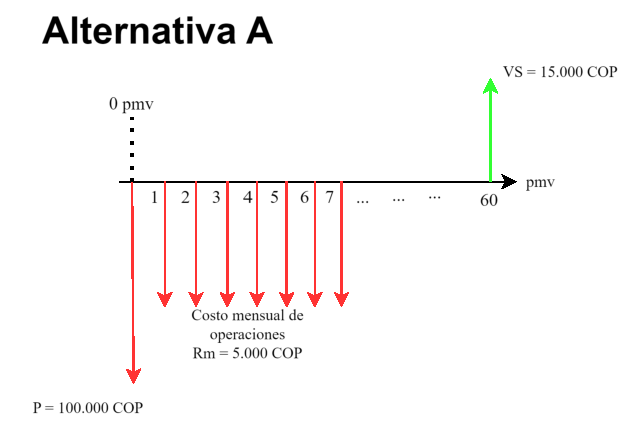
\includegraphics[trim=-5 -5 -5 -5, width=10.5cm, keepaspectratio]{10_Capitulo/img/ejemplos/PDFs/1/Ejemplo_1_A.pdf}}\\ \hline
		\multicolumn{3}{|c|}{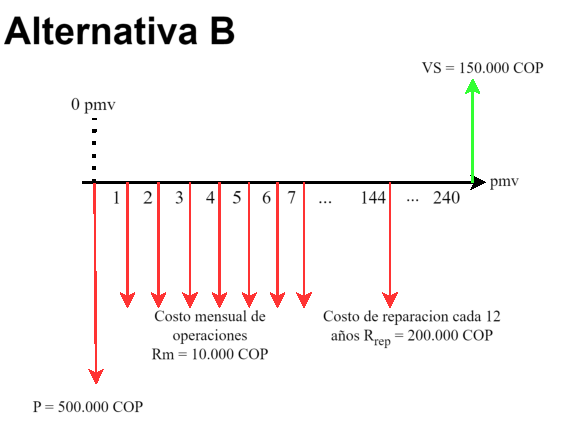
\includegraphics[trim=-5 -5 -5 -5, width=10.5cm, keepaspectratio]{10_Capitulo/img/ejemplos/PDFs/1/Ejemplo_1_B.pdf}}\\ \hline
		%%%%%%%%%%%%% FIN INSERCIÓN DE IMAGEN
		%%%%%FIN FLUJO DE CAJA



		%%%%% INICIO DECLARACIÓN FORMULAS
		%%%%%%%%%%% INICIO TITULO
		\rowcolor[HTML]{FFB183}
		\multicolumn{3}{|c|}{\cellcolor[HTML]{FFB183}\textbf{4. Declaración de fórmulas}}                                                                                    \\ \hline
		%%%%%%%%%%% FIN TITULO
		%%%%%%%%%%% INICIO MATEMÁTICAS

		\multicolumn{3}{|c|}{$VP=R\frac{1-(1+i)^{-n}}{i} \text{ Valor presente serie uniforme vencida}$}\\ 
		\multicolumn{3}{|c|}{$VF=R\frac{(1+i)^{n}-1}{i} \text{ Valor futuro serie uniforme vencida}$}\\
		\multicolumn{3}{|c|}{$CAUE = \sum Ingresos_{anualizados} - \sum Egresos_{anualizados} \text{ CAUE expresado como una sumatoria}$}\\
		\hline
		%%%%%%%%%% FIN MATEMÁTICAS
		%%%%%% INICIO DESARROLLO MATEMÁTICO
		\rowcolor[HTML]{FFB183}
		%%%%%%%%%%INICIO TITULO
		\multicolumn{3}{|c|}{\cellcolor[HTML]{FFB183}\textbf{5. Desarrollo matemático}}                                                                                      \\ \hline
		%%%%%%%%%% FIN TITULO
		%%%%%%%%%% INICIO MATEMÁTICAS
        Alternativa A & \multicolumn{2}{c|}{Alternativa B} \\ \hline
        
		Pasar el costo de operacion de $R_m$ a $R_a$: & \multicolumn{2}{c|}{Pago año 12 ($R_{rep}$) en valor presente} \\
  
		$R_a = {5{.}000*\frac{(1+0,025)^{12}-1}{0,025} = 68{.}978 COP}$ & \multicolumn{2}{c|}{${VP=200	{.}000(1 + 0,34489)^{-12} =  5{.}712}COP$}\\
  
        $ $  & \multicolumn{2}{c|}{}\\
        
		Dividir los 100.000 en 5 pagos anuales uniformes: & \multicolumn{2}{c|} {Nuevo P}\\
  
		${R_1={100{.}000} * \frac{0,34489}{1-(1+0,34489)^{-5}} = 44{.}633}COP $  & \multicolumn{2}{c|}{P = $500{.}000COP + 5{.}712COP = 505{.}712COP$}\\

        $ $  & \multicolumn{2}{c|}{}\\
  
		Dividir los 15.000 en 5 pagos anuales uniformes &\multicolumn{2}{c|} {dividir los 505.712 en 20 pagos anuales}\\
  
		$R_2={15{.}000}* \frac{0,34489}{(1+0,34489)^{5}-1} = 1{.}522COP $ & \multicolumn{2}{c|}{${R_1={505{.}712} * \frac{0,34489}{1-(1+0,34489)^{-5}} = 174{.}882 }COP$}  \\ 

        $ $  & \multicolumn{2}{c|}{}\\
  
		CAUE alternativa A &\multicolumn{2}{c|}{Cuota anual valor salvamento}\\ 
		$CAUE_{A} = 1.522-44.633-68.978$ &\multicolumn{2}{c|}{${R_2={150{.}000}* \frac{0,34489}{(1+0,34489)^{20}-1} = 138COP }$}\\ 

        $ $  & \multicolumn{2}{c|}{}\\
  
		$CAUE_{A} = -112.089 COP$ &\multicolumn{2}{c|}{Pasar el costo de operacion de $R_m$ a $R_a$}\\ 
		&\multicolumn{2}{c|}{$R_a = {10{.}000*\frac{1,025^{12}-1}{0,025} = 137{.}956 }COP$} \\ 

        $ $  & \multicolumn{2}{c|}{}\\
  
		& \multicolumn{2}{c|}{CAUE alternativa B} \\ 
		&\multicolumn{2}{c|}{$CAUE_{B} = 138-174.882-137.956$}\\ 
		&\multicolumn{2}{c|}{$CAUE_{B} = -312.700COP$} \\ \hline
		%%%%%%%%%% FIN MATEMÁTICAS
		%%%%%% FIN DESARROLLO MATEMÁTICO

		\rowcolor[HTML]{FFB183}
		\multicolumn{3}{|c|}{\cellcolor[HTML]{FFB183}\textbf{6. Respuesta}}    \\ \hline

		\multicolumn{3}{|c|}{La alternativa que representa menores perdidas es la A.} \\ \hline
	\end{longtable}
	%Se crean dos lineas en blanco para que no quede el siguiente texto tan pegado
	%\newline \newline
\end{center}
%%%%%%%%%%%%%%%%%%%%%%%%%%FIN EJERCICIO X %%%%%%%%%%%%%%%%%%%%%%%%%%%

%%%%%%%%%% NO OLVIDAR COLOCAR ESTE COMENTARIO CON EL NUMERO DE EJERCICIO %%%%%%%%%%%%%
%%%%%%%%%%%%%%%%%%% EJERCICIO 2 %%%%%%
%%Text bf para negrilla , el \\ es para el salto de linea.
%%El primer \\ hace un espacio en el texto y el 2 \\ crea otro espacio
\textbf{Ejemplo 2}\newline
El jefe de producción de una fábrica debe decidir entre dos máquinas A y B. Las características de cada una son: \\
\begin{center}
		\begin{tabular}{|c|c|c|c|c|}
			\hline
			\rowcolor[HTML]{FFB183}
			\textbf{Maq.} & \textbf{P} & \textbf{n} & \textbf{VS} & \textbf{$R_a$} \\ \hline
			A            & 800.000 COP   & 3 años     & 200.000 COP    & 25.000 COP       \\ \hline
			B            & 600.000 COP   & 2 años     & 150.000 COP    & 30.000 COP       \\ \hline
		\end{tabular}
\end{center}

Con una tasa del 36\% nominal anual año vencido, determinar la mejor alternativa.

\textbf{Solución.}\\
\begin{center}
	\renewcommand{\arraystretch}{1.5}% Margenes de las celdas
	%Creación de la cuadricula
	\begin{longtable}[H]{|c|c|c|}
		%Creamos una linea horizontal
		\hline
		%Definimos el color de la primera fila
		\rowcolor[HTML]{FFB183}
		%%%%% INICIO ASIGNACIÓN FECHA FOCAL %%%%%%%
		%%%%%%%%%% INICIO TITULO
		%Lo que se hace aquí es mezclar las 3 columnas en una sola
		\multicolumn{3}{|c|}{\cellcolor[HTML]{FFB183}\textbf{1. Asignación período focal}}   \\ \hline
		%%%%%%%%%% FIN TITULO
		%%%%% INICIO DECLARACIÓN DE VARIABLES %%%%%%%
		\multicolumn{3}{|c|}{$pf : 0  \textit{ pav }$} \\ \hline
		%Definimos el color de la primera fila
		\rowcolor[HTML]{FFB183}
		%%%%% INICIO DECLARACIÓN DE VARIABLES %%%%%%%
		%%%%%%%%%% INICIO TITULO
		\multicolumn{3}{|c|}{\cellcolor[HTML]{FFB183}\textbf{2. Declaración de variables}}                                                                                   \\ \hline
		%%%%%%%%%% FIN TITULO
		%%%%%%%%%% INICIO SUBTITULO
		\cellcolor[HTML]{FFB183}\textbf{Valores monetarios}    & 
		\cellcolor[HTML]{FFB183}\textbf{Valores no monetarios} &
		\cellcolor[HTML]{FFB183}\textbf{Incógnitas}  \\ \hline
		%%%%%%%%%% FIN SUBTITULO
		%%%%%%%%%% INICIO DE MATEMÁTICAS
		{Alternativa A} & \multicolumn{1}{|c|}{Alternativa A} & \multicolumn{1}{|c|}{Alternativa A}\\
    $P = 800{.}000\text{ COP}$ & $n_A =  3 \textit{ pav }$ & $CAUE_A =  \text{? COP}$\\
    $VS =  200{.}000\text{ COP}$ & $i_a= 36\% \textit{ pav }$ & \\
    $R_a = 25{.}000\text{ COP}$ & &\\
    {Alternativa B} & \multicolumn{1}{|c|}{Alternativa B} & \multicolumn{1}{|c|}{Alternativa B}\\
    $P = 600{.}000\text{ COP}$ & $n_B =  2 \textit{ pav }$& $CAUE_B =  \text{? COP}$\\
    $VS =  150{.}000\text{ COP}$& $i_b= 36\% \textit{ pav }$ & \\
    $R_b = 30{.}000\text{ COP}$& & \\\hline
		%%%%%%%%%% FIN DE MATEMÁTICAS
		%%%%% FIN DECLARACIÓN DE VARIABLES


		%%%%% INICIO FLUJO DE CAJA
		\rowcolor[HTML]{FFB183}
		\multicolumn{3}{|c|}{\cellcolor[HTML]{FFB183}\textbf{3. Diagrama de flujo de caja}}\\ 
        \hline
		%Mezclamos 3 columnas y pondremos el dibujo
		%%%%%%%%%%%%% INSERCIÓN DE LA IMAGEN
		
		\multicolumn{3}{|c|}{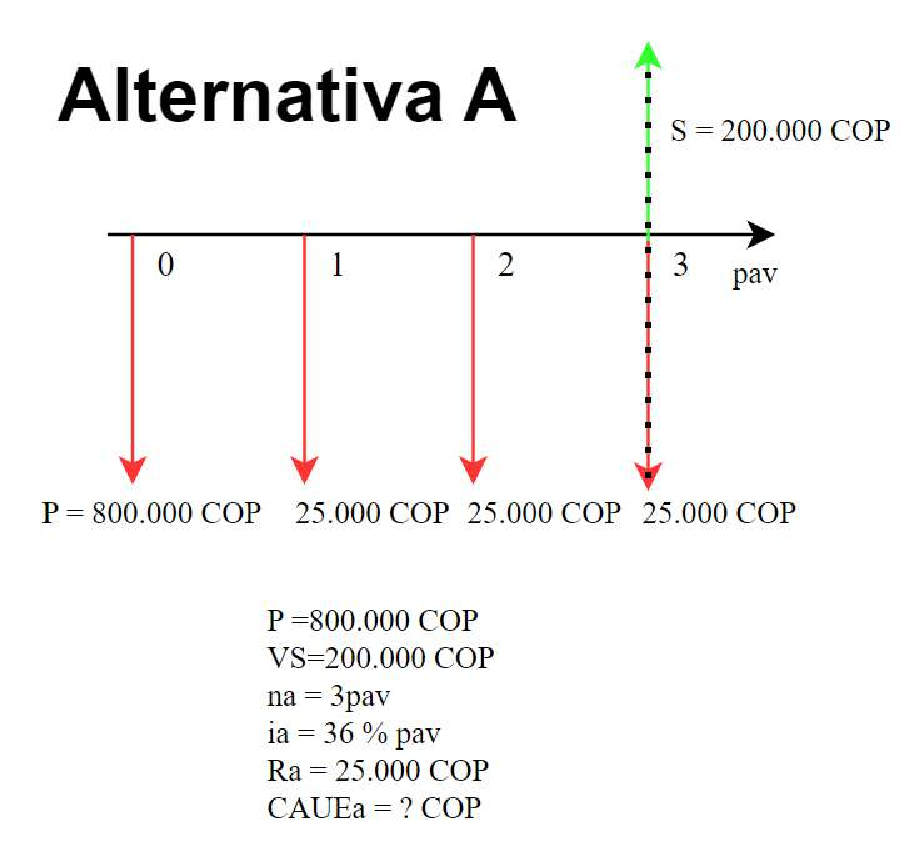
\includegraphics[trim=-5 -5 -5 -5, width=10.5cm, keepaspectratio]{10_Capitulo/img/ejemplos/PDFs/2/Ejemplo_2_A.pdf}}\\ \hline
		\multicolumn{3}{|c|}{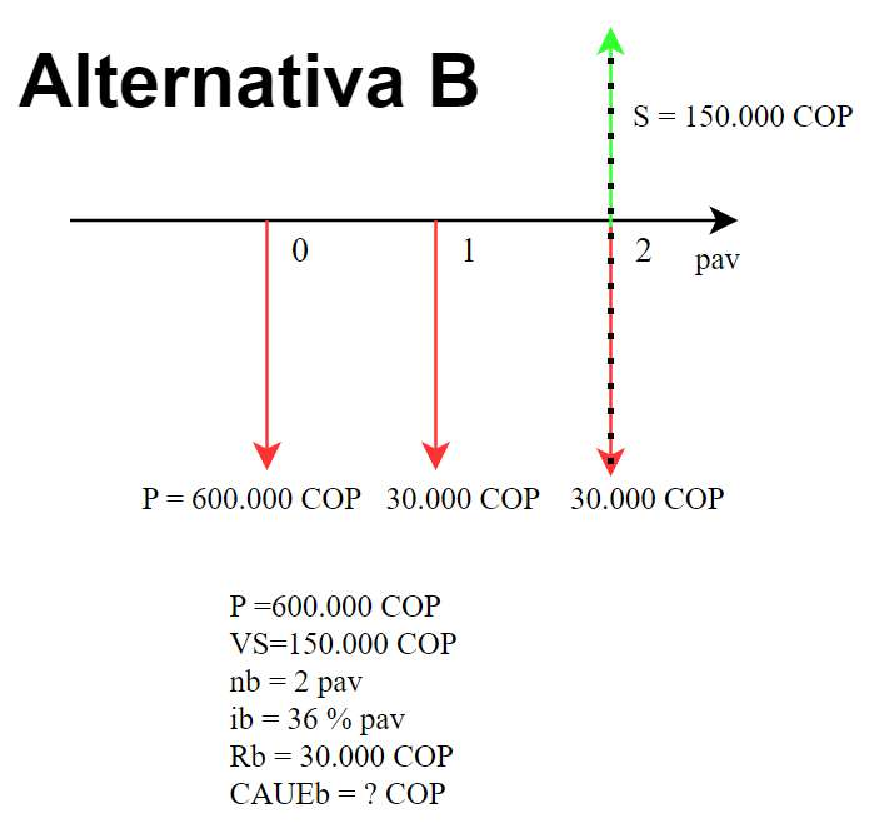
\includegraphics[trim=-5 -5 -5 -5, width=10.5cm, keepaspectratio]{10_Capitulo/img/ejemplos/PDFs/2/Ejemplo_2_B.pdf}}\\ \hline
		%%%%%%%%%%%%% FIN INSERCIÓN DE IMAGEN
		%%%%%FIN FLUJO DE CAJA

		%%%%% INICIO DECLARACIÓN FORMULAS
		%%%%%%%%%%% INICIO TITULO
		\rowcolor[HTML]{FFB183}
		\multicolumn{3}{|c|}{\cellcolor[HTML]{FFB183}\textbf{4. Declaración de fórmulas}} \\ \hline
		%%%%%%%%%%% FIN TITULO
  
		%%%%%%%%%%% INICIO MATEMÁTICAS
		\multicolumn{3}{|c|}{$VP=R\frac{1-(1+i)^{-n}}{i} \text{ Valor presente serie uniforme vencida}$}\\ 
		\multicolumn{3}{|c|}{$VF=R\frac{(1+i)^{n}-1}{i} \text{ Valor futuro serie uniforme vencida}$}\\
		\hline
		%%%%%%%%%% FIN MATEMÁTICAS
  
		%%%%%% INICIO DESARROLLO MATEMÁTICO
		\rowcolor[HTML]{FFB183}
		%%%%%%%%%%INICIO TITULO
		\multicolumn{3}{|c|}{\cellcolor[HTML]{FFB183}\textbf{5. Desarrollo matemático}}   \\ \hline
		%%%%%%%%%% FIN TITULO
		%%%%%%%%%% INICIO MATEMÁTICAS
  
		Alternativa A & \multicolumn{2}{c|}{Alternativa B}\\ \hline
  
		Dividir los 800.000 en 3 pagos anuales uniformes & \multicolumn{2}{c|}{Dividir los 600.000 en 2 pagos anuales uniformes} \\
  
		${R_1={800{.}000} * \frac{0,36}{1-(1+0,36)^{-3}} = 478{.}041{,}809}COP $  & \multicolumn{2}{c|}{  ${R_1={600{.}000} * \frac{0,36}{1-(1+0,36)^{-2}} = 470{.}237{,}288}COP $ }\\

        $ $  & \multicolumn{2}{c|}{}\\
        
        Dividir los 200.000 en 3 pagos anuales uniformes & \multicolumn{2}{c|}{Dividir los 150.000 en 2 pagos anuales} \\
  
		${R_2={200{.}000} * \frac{0,36}{(1+0,36)^{-3}-1} = 47{.}510{,}452}COP $  & \multicolumn{2}{c|}{  ${R_2={150{.}000} * \frac{0,36}{(1+0,36)^{-2}-1} = 63{.}559{,}322}COP $}\\

        $ $  & \multicolumn{2}{c|}{}\\
        
        $CAUE_{A} = -478{.}041,809 - 25.000 + 47{.}510,452 $ & \multicolumn{2}{c|}{
        $CAUE_{B} = -470{.}237,288 - 30{.}000 + 63{.}559,322 $
        }\\

        $ $  & \multicolumn{2}{c|}{}\\

        $CAUE_{A} = -455{.}531,357 COP$ & \multicolumn{2}{c|}{
        $CAUE_{B} = -436{.}677,966 COP$
        }\\

		\hline
		%%%%%%%%%% FIN MATEMÁTICAS
		%%%%%% FIN DESARROLLO MATEMÁTICO

		\rowcolor[HTML]{FFB183}
		\multicolumn{3}{|c|}{\cellcolor[HTML]{FFB183}\textbf{6. Respuesta}}    \\ \hline

		\multicolumn{3}{|c|}{La alternativa que representa menores perdidad es la B.} \\ 
		\hline
	\end{longtable}
	%Se crean dos lineas en blanco para que no quede el siguiente texto tan pegado
	%\newline \newline
\end{center}
%%%%%%%%%%%%%%%%%%%%%%%%%%FIN EJERCICIO X %%%%%%%%%%%%%%%%%%%%%%%%%%%




%%%%%%%%%%% NO OLVIDAR COLOCAR ESTE COMENTARIO CON EL NUMERO DE EJERCICIO %%%%%%%%%%%%%
%%%%%%%%%%%%%%%%%%% EJERCICIO 3 %%%%%%
%%Text bf para negrilla , el \\ es para el salto de linea.
%%El primer \\ hace un espacio en el texto y el 2 \\ crea otro espacio
\textbf{Ejemplo 3}\newline
Se plantea la construcción de un puente y se han presentado dos proyectos, el primero es un puente colgante a un costo de 850.000.000 COP, cada año habrá que darle mantenimiento a la plataforma de asfalto a un costo de 3.000.000 COP, se estima que las reparaciones serán cada vez mayores y que éstas aumentarán de precio todos los años en 2.000.000 COP y cada 5 años habrá que cambiar los cables que sostienen el puente a un costo fijo de 100.000.000 COP, el segundo proyecto es un puente en concreto a un costo de 900.000.000 COP, cada 3 años habrá que reacondicionar las bases a un costo de 25.000.000 COP, el costo anual de mantenimiento se puede considerara fijo en 5.000.000 COP. Con una tasa del 24\% determinar la mejor alternativa.

\textbf{Solución.}\\
\begin{center}

	\renewcommand{\arraystretch}{1.5}% Margenes de las celdas
	%Creación de la cuadricula
	\begin{longtable}{|c|c|c|}
		%Creamos una linea horizontal
		\hline
		%Definimos el color de la primera fila
		\rowcolor[HTML]{FFB183}
		%%%%% INICIO ASIGNACIÓN FECHA FOCAL %%%%%%%
		%%%%%%%%%% INICIO TITULO
		%Lo que se hace aquí es mezclar las 3 columnas en una sola
		\multicolumn{3}{|c|}{\cellcolor[HTML]{FFB183}\textbf{1. Asignación período focal}}   \\ \hline
		%%%%%%%%%% FIN TITULO
		%%%%% INICIO DECLARACIÓN DE VARIABLES %%%%%%%
		\multicolumn{3}{|c|}{$pf : 0 pmv$} \\ \hline
		%Definimos el color de la primera fila
		\rowcolor[HTML]{FFB183}
		%%%%% INICIO DECLARACIÓN DE VARIABLES %%%%%%%
		%%%%%%%%%% INICIO TITULO
		\multicolumn{3}{|c|}{\cellcolor[HTML]{FFB183}\textbf{2. Declaración de variables}}\\ \hline
		%%%%%%%%%% FIN TITULO
		%%%%%%%%%% INICIO SUBTITULO
		\multicolumn{1}{|c|}{\cellcolor[HTML]{FFB183}\textbf{Variables monetarias}}    &
		\multicolumn{1}{c|}{\cellcolor[HTML]{FFB183}\textbf{Variables conceptuales}} &
		\multicolumn{1}{c|}{\cellcolor[HTML]{FFB183}\textbf{Incógnitas}} \\ \hline
		%%%%%%%%%% FIN SUBTITULO
		%%%%%%%%%% INICIO DE MATEMÁTICAS
        $P_A = 850{.}000{.}000\text{ COP}$ & $i = \text{24\% pav}$ & $CAUE_A =  \text{? COP}$ \\
		$R_m =  3{.}000{.}000\text{ + 2.000.000 *n COP}$ & $n_A = \text{5 pav}$ & $CAUE_B =  \text{? COP}$ \\
		$PR = 100{.}000{.}000\text{ COP}$ & $n_B = \text{3 pav}$ &  \\ 
		$P_B = 900{.}000{.}000\text{ COP}$ &  & \\ 
		$CMO = 25{.}000{.}000\text{ COP}$ &  & \\
		$VS =  5{.}000{.}000\text{ COP}$ & & \\ \hline
		%%%%%%%%%% FIN DE MATEMÁTICAS
		%%%%% FIN DECLARACIÓN DE VARIABLES
		%%%%% INICIO FLUJO DE CAJA
		\rowcolor[HTML]{FFB183}
		\multicolumn{3}{|c|}{\cellcolor[HTML]{FFB183}\textbf{3. Diagrama de flujo de caja}}                                                                                  \\ \hline
		%%%%%%%%%%%%% INSERCIÓN DE LA IMAGEN
		\multicolumn{3}{|c|}{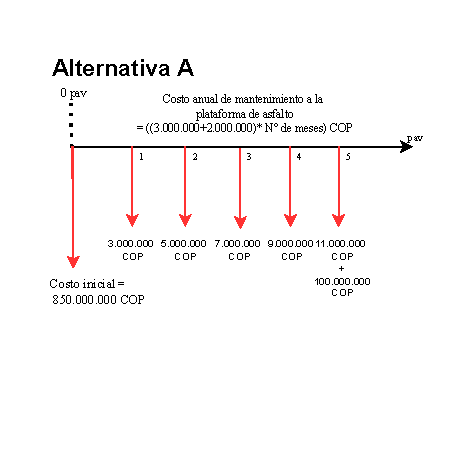
\includegraphics[trim=-5 -5 -5 -5, width=10.5cm, keepaspectratio]{10_Capitulo/img/ejemplos/PDFs/3/Ejemplo_3_A.pdf}}\\ \hline
		\multicolumn{3}{|c|}{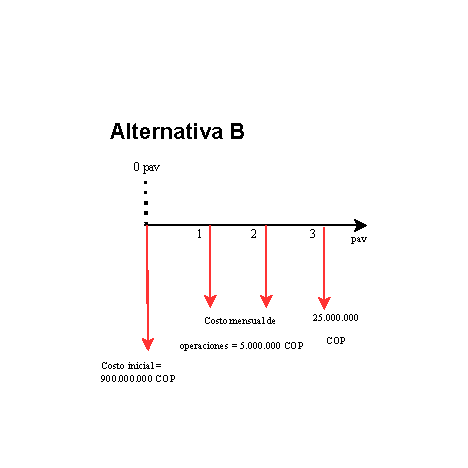
\includegraphics[trim=-5 -5 -5 -5, width=10.5cm, keepaspectratio]{10_Capitulo/img/ejemplos/PDFs/3/Ejemplo_3_B.pdf}}\\ \hline
		%%%%%%%%%%%%% FIN INSERCIÓN DE IMAGEN
		%%%%%FIN FLUJO DE CAJA

		%%%%% INICIO DECLARACIÓN FORMULAS
		%%%%%%%%%%% INICIO TITULO
		\rowcolor[HTML]{FFB183}
		\multicolumn{3}{|c|}{\cellcolor[HTML]{FFB183}\textbf{4. Declaración de fórmulas}}                                                                                    \\ \hline
		%%%%%%%%%%% FIN TITULO
		%%%%%%%%%%% INICIO MATEMÁTICAS
		\multicolumn{3}{|c|}{$VP=R\frac{1-(1+i)^{-n}}{i} \text{ Valor presente serie uniforme vencida}$}\\ 
		\multicolumn{3}{|c|}{$VF=R\frac{(1+i)^{n}-1}{i} \text{ Valor futuro serie uniforme vencida}$}\\
		\multicolumn{3}{|c|}{$CAUE = \sum Ingresos_{anualizados} - \sum Egresos_{anualizados} \text{ CAUE expresado como una sumatoria}$}\\
		\hline                                         
		%%%%%%%%%% FIN MATEMÁTICAS
		%%%%%% INICIO DESARROLLO MATEMÁTICO
		\rowcolor[HTML]{FFB183}
		%%%%%%%%%%INICIO TITULO
		\multicolumn{3}{|c|}{\cellcolor[HTML]{FFB183}\textbf{5. Desarrollo matemático}}\\ \hline
		%%%%%%%%%% FIN TITULO
		%%%%%%%%%% INICIO MATEMÁTICAS
		
		Alternativa A & \multicolumn{2}{c|}{Alternativa B}\\ \hline
  
		Dividir los 100.000.000 en 5 pagos anuales uniformes & \multicolumn{2}{c|}{Dividir los 25.000.000 en 3 pagos anuales uniformes} \\
  
		${R={100{.}000{.}000} * \frac{0,24}{1-(1+0,24)^{5}} = 8{.}186{.}585}COP $  & \multicolumn{2}{c|}{  ${R={25{.}000{.}000} * \frac{0,24}{1-(1+0,24)^{3}} = 3{.}146{.}923}COP $ }\\

        $ $  & \multicolumn{2}{c|}{}\\
        
        CAUE Alternativa A & \multicolumn{2}{c|}{CAUE Alternativa B} \\

        $ $  & \multicolumn{2}{c|}{}\\
        
        $CAUE_{A} = -33{.}000{.}000 - 8{.}186{.}585$ & \multicolumn{2}{c|}{
        $CAUE_{B} = -5{.}000{.}000 - 3{.}146{.}923$
        }\\

        $ $  & \multicolumn{2}{c|}{}\\

        $CAUE_{A} = -41{.}186{.}585 COP$ & \multicolumn{2}{c|}{
        $CAUE_{B} = -8{.}146{.}923 COP$
        }\\

		\hline

		%%%%%%%%%% FIN MATEMÁTICAS
		%%%%%% FIN DESARROLLO MATEMÁTICO
		%%%%% INICIO RESPUESTA
		\rowcolor[HTML]{FFB183}
		\multicolumn{3}{|c|}{\cellcolor[HTML]{FFB183}\textbf{6. Respuesta}}    \\ \hline

		\multicolumn{3}{|c|}{La alternativa que representa menores perdidas es la B.} \\ 
        \hline
		%%%%% FIN RESPUESTA
		
	\end{longtable}
	%Se crean dos lineas en blanco para que no quede el siguiente texto tan pegado
	%\newline \newline
\end{center}
%%%%%%%%%%%%%%%%%%%%%%%%%%FIN EJERCICIO X %%%%%%%%%%%%%%%%%%%%%%%%%%%
